\documentclass[11pt]{beamer}
\usepackage[utf8]{inputenc}
\usepackage[spanish]{babel}
\usepackage{amsmath}
\usepackage{physics}
\usepackage{amsfonts}
\usepackage{amssymb}
\usepackage{graphicx}
\usepackage{ragged2e}
\usepackage{hyperref}
\usepackage{float}
\usepackage{url}
\usepackage{caption}
\usepackage{csquotes}
\usepackage{subfigure}
\usepackage{multicol}
\usepackage[backend=bibtex, sorting=none]{biblatex}
\addbibresource{biblio/referencias.bib}

\usetheme{Antibes}
\setbeamertemplate{footline}[frame number]
\newcommand{\celda}[1]{
	\begin{minipage}{2.5cm}
		\vspace{5mm}
		#1
		\vspace{5mm}
	\end{minipage}
}


\author[José Fernando Tobías Buelvas]{JOSÉ FERNANDO TOBÍAS BUELVAS\inst{1} }
\title[Oscilaciones magnéticas en estructuras basadas en grafeno]{OSCILACIONES MAGNÉTICAS EN ESTRUCTURAS BASADAS EN GRAFENO}
\date{2022}
\logo{
\includegraphics[scale=0.04]{graficas/logo_acreditacion.png}}
\titlegraphic{
\includegraphics[width=1.2cm]{graficas/logo_fisica.jpg}}
\institute[UA]{
	\inst{1}
		Universidad del Atlántico. Programa de Física.\\Facultad de Ciencias Básicas.\\
		\vspace{2mm}}

\AtBeginSection[]
{
	\begin{frame}<beamer>{Contenido}
		\tableofcontents[currentsection,currentsubsection]
	\end{frame}
}


\begin{document}
	\small
	\begin{frame}
		\maketitle
	\end{frame}

	\begin{frame}{Contenido}
		\tableofcontents
	\end{frame}

	\section{Resumen}
		\begin{frame}{Resumen}
%		\begin{multicols}{2}
%			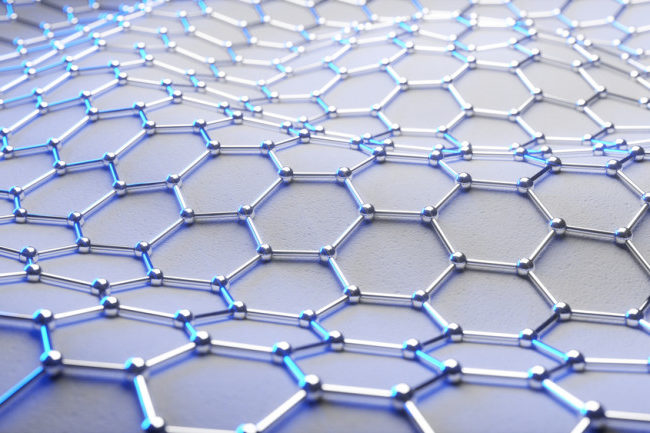
\includegraphics[width=5.2cm,height=3.8cm]{graficas/graphene.jpg}
		\justifying
			El grafeno (red bidimensional de átomos de carbono), catalogado como “el material del futuro”, ha sido objeto de estudio para la comunidad cient\'ifica debido a sus propiedades opto-electrónicas de gran inter\'es.\\
			\vspace{0.5cm}
			El presente trabajo de grado describe el comportamiento oscilatorio de la conductividad el\'ectrica como funci\'on de un campo magnético aplicado
			y su dependencia con la temperatura.
%			\end{multicols}
		\end{frame}

	\section{Planteamiento}
		\begin{frame}{Planteamiento y justificación del problema.}
			\justifying
			El grafeno exhibe propiedades que lo hacen muy interesante para la ciencia y para aplicaciones tecnológicas.\\
			Cada vez hay más dispositivos basados en grafeno y se hace necesario tener un mayor entendimiento teórico
			de las propiedades físicas de las estructuras basadas en grafeno.\\
			\vspace{0.5cm}
			En este contexto, el presente trabajo realiza una descripción teórica de la conductividad eléctrica
			en un sistema de una monocapa de grafeno colocada sobre un cristal de nitruro de Boro hexagonal (hBN).
		\end{frame}

		\begin{frame}{Planteamiento del problema}
			\justifying
			Con base en lo expuesto anteriormente, se plantea el siguente interrogante:
			\begin{itemize}
				\item ¿Cuál es la dependencia con la temperatura de las oscilaciones magnéticas de la conductividad eléctrica?
			\end{itemize}
		\end{frame}


	\section{Objetivos}
		\begin{frame}{Objetivo general}
			\justifying
			\begin{itemize}
    		\item Estudiar oscilaciones de la conductividad eléctrica en estructuras basadas en grafeno como función del campo magnético aplicado.
				\end{itemize}
		\end{frame}

		\begin{frame}{Objetivos específicos}
			\justifying
			\begin{enumerate}
			    \item Resolver la ecuación de Schrödinger para una estructura sustrato-grafeno en presencia de un campo magnético externo.
			    \item<2-> Determinar la densidad de estado del sistema.
			    \item<3-> Obtener la conductividad eléctrica del sistema.
			    \item<4-> Calcular la dependencia con respecto a la temperatura de las oscilaciones magnéticas en estructuras basadas en grafeno.
			\end{enumerate}

		\end{frame}

	\section{Metodología}
		\begin{frame}{Metodología}
			\justifying
			\begin{enumerate}
				\item Estudiar las propiedades y la f\'isica general del grafeno.
				\item<2-> A partir del Hamiltoniano del sistema, resolver la ecuaci\'on de Schrödinger.
				\item<3-> Hallar los niveles de Landau del espectro de energ\'ia.
				\item<4-> Determinar la funci\'on de Green asociada a los estados de banda del sistema.
				\item<5-> Determinar la densidad de estados del sistema.
				\item<6-> Estudiar el comportamiento oscilatorio de la conductividad el\'ectrica como funci\'on de la temperatura.
				\item<7-> Realizar c\'alculos num\'ericos.
			\end{enumerate}
		\end{frame}

	\section{Introducción}
\justifying

\begin{frame}{Grafeno}
	Es una de las formas alotrópicas del carbono.

	\begin{figure}
		\subfigure[Propiedades del grafeno]{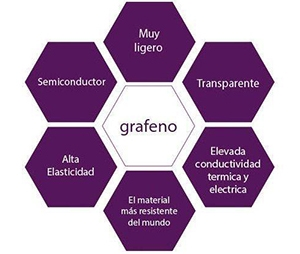
\includegraphics[width=4cm]{graficas/propiedadesGrafeno.jpg}}
		\subfigure[Alótropos del carbono]{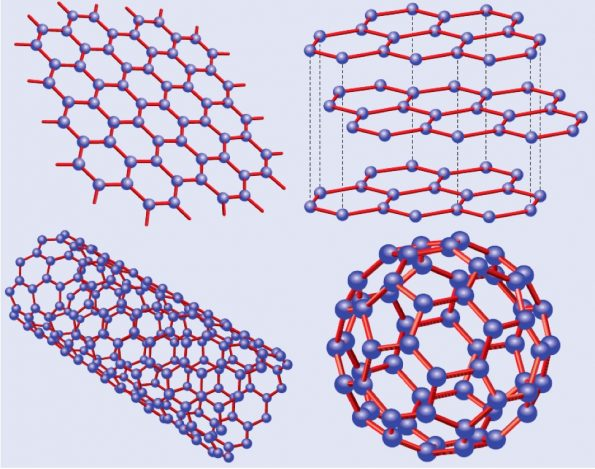
\includegraphics[width=4cm]{graficas/alotropo.jpg}}
		\caption{Grafeno, \textit{Tomado de }\cite{Neto2006} }
	\end{figure}
\end{frame}

\begin{frame}
	Las oscilaciones magnéticas son un fenómeno conocido en la física de la materia condensada, generalmente observado a bajas temperaturas.
	En el grafeno, persiste incluso a temperaturas ambiente. Esto se atribuye a la periodicidad de las superredes de grafeno \cite{Kumar2017}.

	\begin{figure}
		\subfigure[Superred de grafeno]{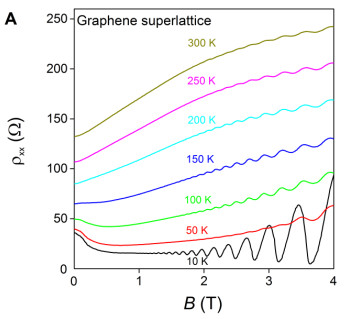
\includegraphics[width=4cm]{graficas/oscilaciones_superred.jpg}}
		\subfigure[grafeno]{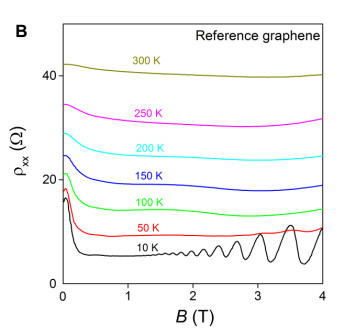
\includegraphics[width=4cm]{graficas/oscilaciones_grafeno.jpg}}
	\caption{$\rho$ vs $B$ a diferentes temperaturas. \textit{Tomadas de \cite{Kumar2017}}}
	\end{figure}
\end{frame}

\begin{frame}
	\begin{multicols}{2}
		Los sistemas electrónicos tambien presentan oscilaciones magnéticas,
		referidos a las mariposas de Hofstadter (HB) \cite{Yu2014}-\cite{Yang2016}.\\
		\vspace{0.5cm}
		Estudios de transporte eléctrico en superredes de grafeno sobre h-BN \cite{Yankowitz2012}
		muestran características de las HB originadas en la superred en un campo magnético \cite{BenShalom2016}.
		\begin{figure}
			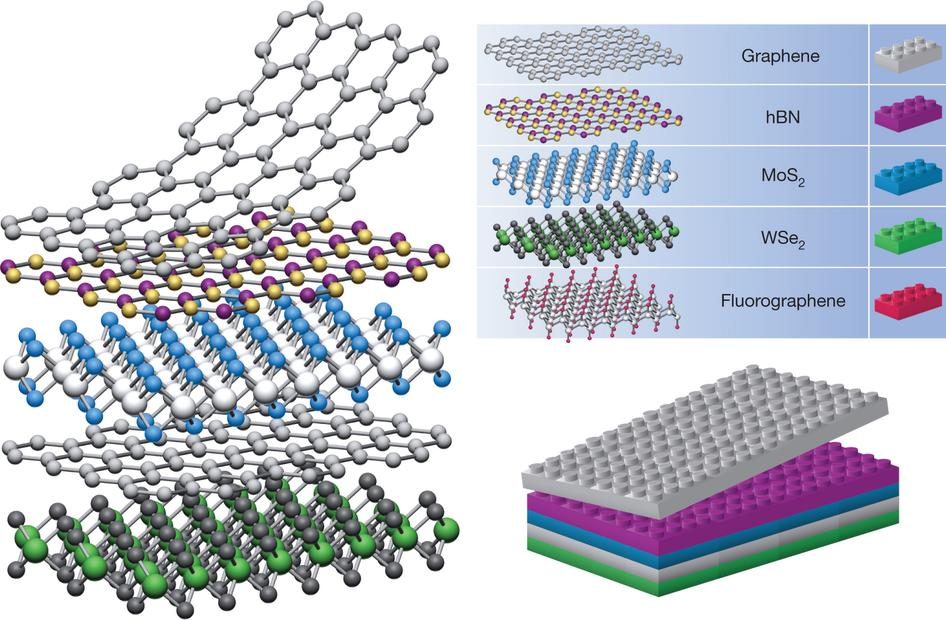
\includegraphics[width=6cm]{graficas/heterostructures.jpg}
			\caption{Superredes de grafeno. \textit{Tomado de} \cite{Geim2013}}
			\label{heterostructures}
		\end{figure}
	\end{multicols}
\end{frame}

	\section{Espectro de energía}

\subsection{Niveles de Landau}
\begin{frame}{Niveles de Landau}
	\begin{multicols}{2}
	\scriptsize{En presencia de un campo magn\'etico, los electrones solo pueden ocupar \'orbitas con estados discretos de energ\'ia, llamados niveles de Landau (L.L. Por sus siglas en ingl\'es).	Estos niveles vienen dados por la ecuaci\'on:
	\begin{equation}
		E_n = \hbar \omega_c (n+\frac{1}{2})
	\end{equation}
	donde $\hbar$ es la constante de planck normalizada, $n\in \mathbb{Z}$ y  $\omega_c=\frac{eB}{mc}$ es la frecuencia del ciclotrón, 
	$e$ es la carga del electrón, $B$ la magnitud del campo magnético, $m$ la masa y $c$ es la velocidad de la luz.}
	\begin{figure}[b!]
		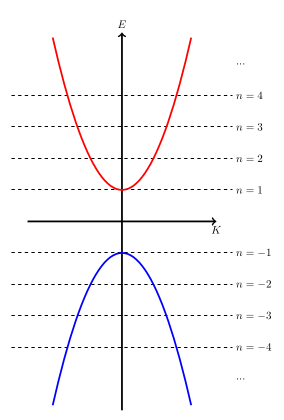
\includegraphics[width=3cm,height=4.5cm]{graficas/LL_material.png}
			\caption{\scriptsize{Niveles de Landau en material convencional}}
	\end{figure}
	\end{multicols}
\end{frame}

\begin{frame}{Niveles de Landau en el grafeno}
	\begin{multicols}{2}
		\scriptsize{En el grafeno, los niveles de Landau se pueden obtener a partir de considerar el hamiltoniano, 
						$\hat{H}=\frac{\hat{\pi}^2}{2m}+V(\vec{r})$ siendo $\pi=\vec{p}-e/c\vec{A}$ y $\vec{A}$ es el potencial vector, de la forma:
			\begin{equation}
					\hat{H} = \sqrt{\frac{2e\hbar B \nu_f}{c}}
					\left( \begin{array}{c c}
							0&\hat{a}\\\hat{a}^\dagger&0
					\end{array} \right)
			\end{equation}
			donde $\hat{a}= \sqrt{c/2e\hbar B}(\pi_x-i\pi_y)$ y 	$\hat{a}^\dagger=\sqrt{c/2e\hbar B}(\pi_x+i\pi_y)$. Resolviendo la ecuación de Schrödinger
			se obtiene que los niveles de energía vienen dados por:
			\begin{equation}
					E_n= \pm \hbar\omega_c \sqrt{n}
			\end{equation}
			donde $\omega_c = \sqrt{2}\nu_f/l_B$ es el ciclotrón cuántico y $l_B = \sqrt{\frac{\hbar c}{e B}}$ es la longitud magnética.}
		\begin{figure}
			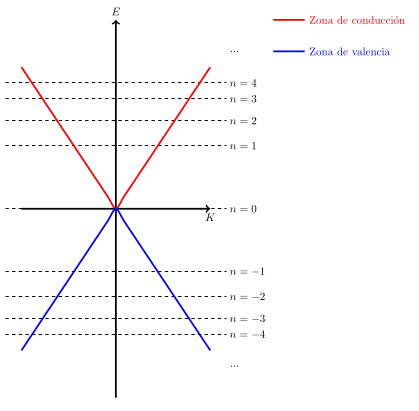
\includegraphics[height=4.5cm]{graficas/LL_grafeno.png}
			\caption{\scriptsize{Niveles de Landau en el grafeno}}
		\end{figure}
	
	\end{multicols}
	\end{frame}
\subsection{Estados de Bloch en grafeno en un campo eléctrico}

\begin{frame}
\end{frame}
\begin{frame}
\end{frame}
\begin{frame}
\end{frame}
\begin{frame}
\end{frame}

\begin{frame}
\end{frame}
\begin{frame}
\end{frame}
\begin{frame}
\end{frame}

	\section[Oscilaciones]{Oscilaciones magnéticas}
\justifying

\subsection{Conductividad longitudinal en una capa de grafeno}

\begin{frame}
  La geometría experimental consiste en una barra de Hall de grafeno
  sobre un sustrato de hBN.\\

  \begin{figure}[h]
      \centering
      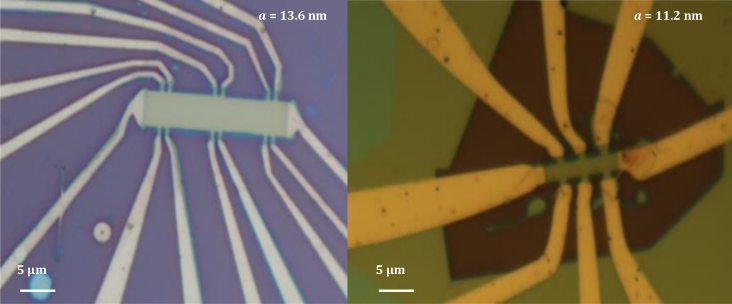
\includegraphics[scale=0.4]{graficas/hall_bar.png}
      \caption{Imágenes ópticas de barra de Hall multiterminal usadas por Kumar et Al. \cite{Kumar2017}}
      \label{Hall_bar}
  \end{figure}
\end{frame}

\begin{frame}
  Para obtener una expresión de la conductividad,
  se usará el enfoque del hamiltoniano de transferencia \cite{Illera2015}.\\
  La tasa de transición de estados se calcula usando la regla de oro de Fermi \cite{Illera2015}-\cite{Sakurai2017}:

  \begin{equation}\label{golden rule}
    d^{2}W_{l\rightarrow r \in D}=\sum_{\eta'}d^{2}W_{\eta,\eta'}=\frac{2\pi}{\hbar}\sum_{\eta'}|t_{\eta,\eta'}|^{2}\rho_{r}(\epsilon')\delta(\epsilon'-\epsilon)d\epsilon',
  \end{equation}

  $t_{\eta,\eta'}$ representa la transición entre los estados $|\eta|$ y $|\eta'|$ y $\rho(\epsilon')$ es la densidad de estados de la derecha.
\end{frame}

\begin{frame}
  La tasa de transición de los estados ocupados de la izquierda a los no ocupados de la derecha
  en el camino entre los dos contactos de la siguiente forma:
  \scriptsize
  \begin{equation}
    \Gamma_{l\rightarrow r}=\frac{2\pi}{\hbar}\sum_{\eta}\int \rho_{l}(\epsilon)f_{l}(\epsilon)\left\lbrace \int\sum_{\eta''}|t_{\eta',\eta''}|^{2}\rho_{r}(\epsilon'')[1-f_{r}(\epsilon'')]\delta(\epsilon''-\epsilon')d\epsilon''\right\rbrace d\epsilon.
  \end{equation}
  \small
  La corriente de transferencia es:
  \begin{equation}
    I=e(\Gamma_{l\rightarrow r}-\Gamma_{r\rightarrow l}).
  \end{equation}
\end{frame}

\begin{frame}
  Considerando simetria en la matriz de salto ($t_{\eta,\eta'} = t_{\eta',\eta}$),
  \begin{equation}
    I=-g\frac{2\pi e}{\hbar}\sum_{\eta'}\int |t_{\eta,\eta'}|^{2}[f(\epsilon)-f(\epsilon-eU_{g})]\textbf{Im}G_{l}^{R}(\epsilon)\mathbf{Im} G_{r}^{R}(\epsilon-eU_{g})d\epsilon,
  \end{equation}
  donde $f$, $g$ y $G_R$ son las funciones de Fermi, la degeneración y la función de Green retardada.
\end{frame}

\begin{frame}
  Los elementos de la matriz de transición se relacionan con la velocidad del electrón,
  $$v_{\eta} = \frac{1}{\hbar}\frac{\partial\zeta}{\partial k_{\eta}},$$
  mediante la relación:

  \begin{equation}
    | t_ {\eta, \eta'} |^ {2} = \frac{2 \pi \hbar^{2} }{L_{\eta} L_{\eta'}}v_{\eta} v_{\eta'}.
  \end{equation}
\end{frame}

\begin{frame}
  La conductividad se obtiene de la siguiente manera:
  \begin{equation}
    \sigma_{xx} = \frac{L_x}{L_y}\left(\frac{dI}{dU_g}\right)_{U_g=0},
  \end{equation}

  \begin{equation}
    \sigma_{xx}=\sigma_{o}\sum_{n,k_{y},\beta}\int |t_{x,x}|^{2}\left(-\frac{\partial f}{\partial\epsilon'}\right)\left[2\textbf{Im}G_{n,k}^{R}(\epsilon')\right]^{2}d\epsilon,
    \label{eq:conductividad}
  \end{equation}

  donde se ha tomado $\rho(\epsilon) = - \frac{1}{\pi}\textbf{Im} G_{R} (\epsilon)$,
  $\sigma_{o} = \frac{2 e^{2} n_{L} L_{x}}{\pi \hbar L_{y}}$,
  $ L_{x (y)} $ son las dimensiones de la muestra y $ n_{L} = \Phi / \Phi_{o} $, ($\Phi_{0} = \frac{2\pi}{\hbar})$.
\end{frame}

\subsection{Oscilaciones magnéticas a altas temperaturas}

\begin{frame}
  A partir de la ecuación \ref{eq:conductividad}, se toma:

  \begin{equation}
    [2\textbf{Im}G^{R}(\epsilon)]^2 = G_{R}^{2}+G_{A}^{2}-2G_{R}G_{A},
    \label{2ImGr2}
  \end{equation}
  $G_A$ es la función avanzada de Green que toma la forma \cite{Vega2016}-\cite{Salazar2016}:
  \begin{equation}
    G_A(\epsilon) = \frac{1}{\epsilon'-\epsilon_n-\Sigma^A(\epsilon)} + \frac{1}{\epsilon'+\epsilon_n-\Sigma^A(\epsilon)},
  \end{equation}
\end{frame}

\begin{frame}
  En una forma compacta $G_R$ y $G_A$ pueden escribirse:\\
  \begin{align}
    G_R(\epsilon) = \frac{2(\epsilon'-i |\textbf{Im}\Sigma|)}{(\epsilon'-i |\textbf{Im}\Sigma|)^2-\epsilon_{n}^{2}}    \qquad G_A(\epsilon) = \frac{2(\epsilon'+i |\textbf{Im}\Sigma|)}{(\epsilon'+i |\textbf{Im}\Sigma|)^2-\epsilon_{n}^{2}}.
  \end{align}

  \vspace{0.5cm}
  donde la función $\Sigma^R(\epsilon) = Re\Sigma(\epsilon)+i Im\Sigma(\epsilon)$ es la autoenergía retardada compleja.
\end{frame}

\begin{frame}
  Usando la fórmula de sumatoria de Poisson:
  \begin{equation}
    \sum_{n=-\infty}^{\infty}F(n) = \textbf{Re}\sum_{r=-\infty}^{\infty}\int_{0}^{\infty}F(y)e^{2\pi i r y}dy,
  \label{Fn}
  \end{equation}
  y aplicando el teorema del residuo, donde los polos est\'an dados por $\pm2i\epsilon|Im\Sigma|/\varepsilon_{a}^{2}$, se obtiene:
  \begin{equation}
    \sum_{n=-\infty}^{\infty}G_R G_A =\textbf{Re} \sum_{r=-\infty}^{\infty}\frac{4\pi}{\epsilon_{f}^{2}}\frac{\epsilon'}{|\textbf{Im}\Sigma|} e^{-4\pi r\frac{\epsilon'|\textbf{Im}\Sigma|}{\epsilon_{f}^{2}}} e^{2\pi i r \frac{\epsilon'^2}{\epsilon_{f}^{2}}}.
    \label{GrGa}
  \end{equation}
\end{frame}

\begin{frame}
  Teniendo en cuenta:
  \begin{equation}
    Res\left(h,z_{0}\right)=\lim_{z\rightarrow z_{0}}\frac{1}{\left(n-1\right)!}\frac{d^{n-1}}{dz^{n-1}}\left\{ \left(z-z_{0}\right)^{n}h\left(z\right)\right\}.
    \label{res}
  \end{equation}

  se obtiene:
  \begin{equation}
    G_{R}^{2}=\frac{4\left(\epsilon'^{2}-2i\epsilon'|Im\Sigma|\right)}{\epsilon_{f}^{4}\left(-\frac{2i\epsilon'|Im\Sigma|}{\epsilon_{f}^{2}}-x^{2}\right)^{2}},
    \label{Gr2}
  \end{equation}
\end{frame}

\begin{frame}
  Aplicando la ecuaci\'on (\ref{Fn}) se tiene:
  \begin{equation}
    \sum_{n=-\infty}^{\infty}G_{R}^{2}=\sum_{r=-\infty}^{\infty}\frac{4\left(\epsilon'^{2}-2i\epsilon'|Im\Sigma|\right)}{\epsilon_{f}^{4}}e^{2\pi ir\left(\frac{\epsilon'^{2}}{\epsilon_{f}^{2}}\right)}\int_{-\infty}^{\infty}\frac{e^{2\pi irx}}{\left[-\frac{2i\epsilon'|Im\Sigma|}{\epsilon_{f}^{2}}-x\right]^{2}}dx.
    \label{Gr22}
  \end{equation}
  Aplicando la expresi\'on (\ref{res}) en la ecuaci\'on (\ref{Gr2}) se obtiene
  \begin{equation}
      \sum_{n=-\infty}^{\infty}G_{R}^{2} =\textbf{Re} \sum_{r=-\infty}^{\infty}\frac{4\pi}{\epsilon_{f}^{2}}\frac{\epsilon'}{|\textbf{Im}\Sigma|} e^{2\pi i r \frac{\epsilon'^2}{\epsilon_{f}^{2}}} e^{-4\pi |r|\frac{\epsilon'|\textbf{Im}\Sigma|}{\epsilon_{f}^{2}}} \left( \frac{4\pi |r|\epsilon'|\textbf{Im}\Sigma|}{\epsilon_{f}^{2}}  \right).
      \label{Gr23}
  \end{equation}
\end{frame}

\begin{frame}
  Igualmente se tiene que
  \begin{equation}
    \sum_{N}^{\infty}G_{A}^{2}=\sum_{r=-\infty}^{\infty}\frac{4\pi\epsilon'}{\epsilon_{f}^{2}|Im\Sigma|}e^{2\pi i\mid r\mid\left(\frac{\epsilon'^{2}}{\epsilon_{f}^{2}}\right)}e^{-\frac{4\pi\mid r\mid\epsilon'|Im\Sigma|}{\epsilon_{f}^{2}}}\left[\frac{4\pi\mid r\mid\epsilon'|Im\Sigma|}{\epsilon_{f}^{2}}\right].
    \label{Ga2}
  \end{equation}
  Sustituyendo (\ref{GrGa}), (\ref{Gr23}) y (\ref{Ga2}) en (\ref{2ImGr2}), se obtiene:

  \begin{equation}
    \left[2ImG_{R}\left(k\right)\right]^{2}=\sum_{r=-\infty}^{\infty}\frac{4\pi\epsilon'}{\epsilon_{f}^{2}\mid Im\Sigma\mid}R_{D}e^{2\pi ir\left(\frac{\epsilon'^{2}}{\epsilon_{f}^{2}}\right)}\left[1+\frac{8\pi\mid r\mid\mid Im\Sigma\mid\epsilon'}{\epsilon_{f}^{2}}\right].
    \label{2ImGr22}
  \end{equation}
\end{frame}

\begin{frame}
  Luego, la conductividad longitudinal toma la forma:
  \begin{equation}
    \sigma_{xx} = g \frac{2 e^2 L_x}{\hbar L_y \epsilon_{f}^{2}} \textbf{Re} \sum_{k,r}\int\left| t_{k,k}\right|^2 G_{xx}(\epsilon,r) \left(-\frac{\partial f}{\partial\epsilon}\right)d\epsilon,
    \label{eq:sigmaxx}
  \end{equation}

  donde $$
      G_{xx}(\epsilon,r) = \frac{\epsilon'}{|\textbf{Im}\Sigma|} e^{2\pi i r \frac{\epsilon'^2}{\epsilon_{f}^{2}}} R_D(\epsilon,r) \left[ 1+8\pi |r| \frac{|\textbf{Im}\Sigma|\epsilon'}{\epsilon_{f}^{2}}\right].
    $$
  $$ R_D(\epsilon,r) = \exp\left( -4\pi |r|\frac{|\textbf{Im}\Sigma|\epsilon'}{\epsilon_{f}^{2}}\right) $$
\end{frame}

\begin{frame}
  Introduciendo el factor $S(\lambda,\delta)$ se puede escribir (\ref{eq:sigmaxx}) de forma compacta:
  \begin{equation}
    S(\lambda,\delta) = \sum_{r=-\infty}^{\infty} e^{-|r|\lambda}\cos\delta r = \frac{\sinh\lambda}{\cosh\lambda-\cos\delta},
  \end{equation}
  donde
  \begin{equation}
    \lambda= \frac{4\pi\epsilon'|\textbf{Im}\Sigma|}{\epsilon_{f}^{2}}
  \end{equation}
  y
  \begin{equation}
    \delta= 2\pi\frac{\epsilon'^2}{\epsilon_{f}^{2}}.
  \end{equation}
\end{frame}

\begin{frame}
  La conductividad se puede escribir como $\sigma_{xx} = \sigma_B+ \sigma_Q$ donde:
  \begin{equation}
    \sigma_B= \sigma_{o}\int d\epsilon N(\zeta)\frac{\epsilon}{|\textbf{Im}\Sigma|}\left(-\frac{\partial f}{\partial\epsilon}\right)S(\lambda,\delta).
    \label{eq:sigmaB}
  \end{equation}
  Por otra parte,
  \begin{equation}
    \sigma_Q= -\sigma_{o}\int d\epsilon N(\zeta)\frac{\epsilon}{|\textbf{Im}\Sigma|}\left(-\frac{\partial f}{\partial\epsilon}\right) \left(\lambda_o \frac{\partial S(\lambda,\delta)}{\partial \lambda}\right),
    \label{eq:sigmaQ}
  \end{equation}
  donde $\lambda_o=8 \pi\epsilon'|\textbf{Im}\Sigma|/\epsilon_{f}^{2}$.
\end{frame}

\begin{frame}
  El parámetro $N(\zeta)$ está relacionado con los estados de Bloch,
  \begin{equation}
    N(\zeta)=\frac{L_{x}L_{y}}{a_{x}\pi^{2} \varepsilon_{f}^{2}}\int_{0}^{a_{x}/2l^{2}}dk_{y} \int_{0}^{2\pi}d\beta|t_{x,x}|^{2}.
  \end{equation}

  Luego, la conductividad longitudinal puede escribirse como:
  \begin{equation}
    \sigma_{xx}=\sigma_{o}\int  N(\zeta)\left(-\frac{\partial f}{\partial\epsilon}\right)\frac{\epsilon}{\mid \textbf{Im}\Sigma\mid}G_{xx}(\delta,\lambda)d\epsilon,
    \label{condxx}
  \end{equation}

  donde $G_{xx}(\delta,\lambda)=\left[ 1-\lambda_{o}\frac{\partial }{\partial\lambda}\right] S(\delta,\lambda)$.
\end{frame}

\begin{frame}
  \begin{figure}[h!]
    \begin{center}
      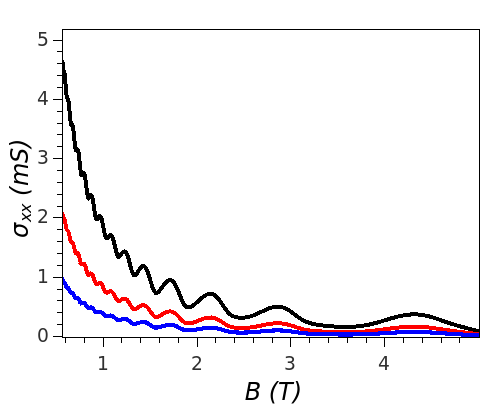
\includegraphics[scale=0.5]{graficas/fig5.png}
      \caption{$\sigma_{xx}$ vs. $B$ para $T = 150 K$ (negra), $T = 200 K$ (roja) y $T = 250 K$ (azul).}
      \label{sigmavsB}
      \centering
    \end{center}
  \end{figure}
\end{frame}

\begin{frame}
  \begin{figure}[h!]
    \begin{center}
      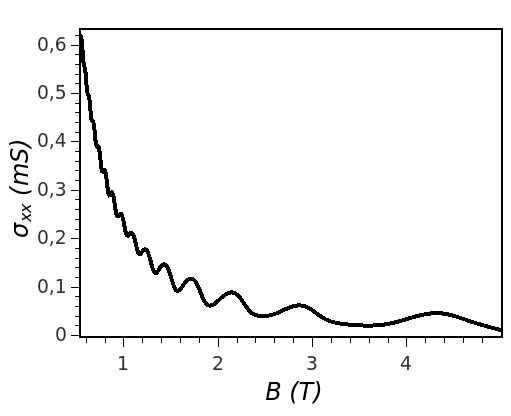
\includegraphics[scale=0.5]{graficas/fig6.png}
      \caption{$\sigma_{xx}$ vs. $B$ ($T = 300 K$).}
      \label{sigma300k}
      \centering
    \end{center}
  \end{figure}
\end{frame}

\begin{frame}
  \begin{figure}[h!]
    \begin{center}
      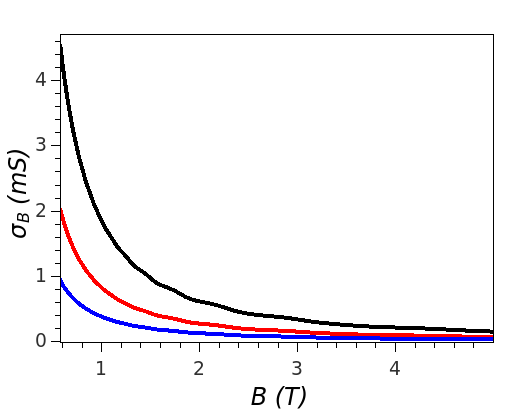
\includegraphics[scale=0.5]{graficas/fig8.png}
      \caption{$\sigma_{B}$ vs. $B$ $T = 150 K$ (negra), $T = 200 K$ (roja) y $T = 250 K$ (azul).}
      \label{cont_Boltz}
      \centering
    \end{center}
  \end{figure}
\end{frame}

\begin{frame}
  \begin{figure}[h!]
    \begin{center}
      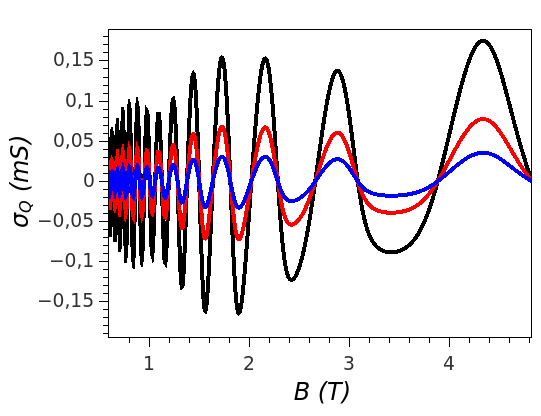
\includegraphics[scale=0.5]{graficas/fig9.png}
      \caption{$\sigma_{Q}$ vs. $B$ $T = 150 K$ (negra), $T = 200 K$ (roja) y $T = 250 K$ (azul).}
      \label{cont_Cuant}
      \centering
    \end{center}
  \end{figure}
\end{frame}

\begin{frame}
  \begin{figure}[h!]
    \begin{center}
      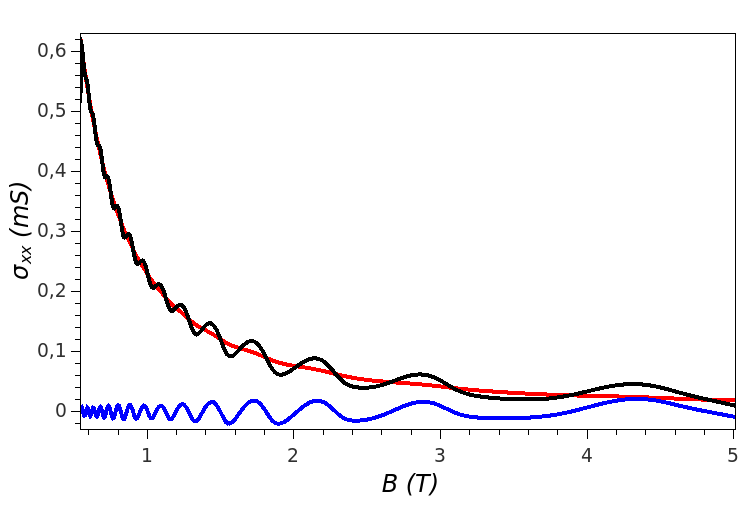
\includegraphics[scale=0.4]{graficas/fig7.png}
      \caption{$\sigma_{xx}$, $\sigma_{B}$ y $\sigma_{Q}$ vs. $B$ ($T = 300 K$).}
      \label{contrib}
      \centering
    \end{center}
  \end{figure}
\end{frame}

\begin{frame}
  Para todos los cálculos, los parámetros utilizados son $v_{f}=1.15\times 10^{6}$ m/s, $a_{x}=a_{y}=a=50$ nm,
  $V_{o}=1\times10^{-6}$ eV, $U_{x}=U_{y}=U_{o}=0.5\times10^{-3}$ eV, $n_{i}=3\times10^{15}$ m$^{-2}$
  y la energía de Fermi $\mu_{o}=100$ meV.\\

  \vspace{0.5cm}

  Las oscilaciones a altas temperaturas debidas a la contribución $\sigma_{Q} $ responden a variaciones periódicas
  del parámetro de desorden, las cuales están determinadas por la variación del factor de forma $ S(\delta,\lambda)$.
\end{frame}

\subsection{Tiempo de relajación del electrón}

\begin{frame}
  La parte imaginaria de la auto energía $\Sigma(\epsilon)$ está relacionada con la dispersión del electrón
  por medio del tiempo de relajación electrónico \cite{Ando1974},
  \begin{equation}
    \frac{\hbar}{\tau} = |\textbf{Im}\Sigma|.
  \end{equation}
  En este trabajo se analiza un modelo de impurezas como potenciales puntuales
  \begin{equation}
    V(\Vec{r}-\Vec{R}) = V_0 \delta(\Vec{r}-\Vec{R}),
  \end{equation}
\end{frame}

\begin{frame}
  Similarmente a como se desarrolló anteriormente, se tiene:
  \begin{equation}
    G_{R}(n,k) = \frac{2(\epsilon' - i|Im\Sigma|)}{(\epsilon' - |Im\Sigma|)^{2} - \epsilon_{n}^{2}},
    \label{GRnk2}
  \end{equation}

  \begin{equation}
    \sum_{n=-\infty}^{\infty}G_{R}=\sum_{r=-\infty}^{\infty}\frac{2(\epsilon' - i|Im\Sigma|)}{\epsilon_{f}^{2}}e^{2\pi ir\left(\frac{\epsilon'^{2}}{\epsilon_{f}^{2}}\right)}\int_{-\infty}^{\infty}\frac{e^{2\pi irx}}{\left[\frac{2i\epsilon'|Im\Sigma|}{\epsilon_{f}^{2}}-x\right]}dx
    \label{GRPoisson}
  \end{equation}
\end{frame}

\begin{frame}
  La parte imaginaria de la autoenergía queda:
  \begin{equation}
    \mid Im\Sigma\mid=\frac{n_{i}L_{x}L_{y}V_{o}^{2}\epsilon'}{a_{x}\pi^{2} \epsilon_{f}^{2}}\sum_{r}\int_{0}^{a_{x}/2l^{2}}dk_{y} \int_{0}^{2\pi}d\beta e^{-\frac{4\pi\epsilon'|Im \Sigma|}{\epsilon_{f}^{2}}}e^{2\pi ir\frac{\epsilon'^{2}}{\epsilon_{f}^{2}}}.
    \label{|ImE|}
  \end{equation}
  de donde se obtiene:
  \begin{equation}
    \frac{\left|\textbf{Im}\Sigma\right|}{\epsilon}=\frac{n_{i}L_{x}L_{y}V_{o}^{2}}{a_{x}\pi^{2} \varepsilon_{f}^{2}}\int_{0}^{a_{x}/2l^{2}}dk_{y} \int_{0}^{2\pi}d\beta S(\delta,\lambda).
    \label{Im/e}
  \end{equation}
\end{frame}

\begin{frame}
  Se puede aproximar la expresión para la parte imaginaria de la autoenergía de la siguiente forma
  \begin{equation}
    \tau(\epsilon)\frac{\epsilon}{\epsilon_{f}}S(\delta,\lambda)=\tau_{o},
    \label{tau}
   \end{equation}
  donde
   \begin{equation}
    \tau_{o}=\frac{\pi\hbar l^{2}\epsilon_{f}}{N_{i}V_{o}^{2}}.
    \label{tau_0}
   \end{equation}
\end{frame}

\begin{frame}
  Se tiene entonces que la contribución de Boltzmann $\sigma_B$ puede escribirse así:
  \begin{equation}
    \sigma_{B}=\sigma_{\tau}\int d\epsilon N(\zeta)\left(-\frac{\partial f}{\partial\epsilon}\right),
  \end{equation}
  donde $ \sigma_{\tau} = \sigma_{o} \tau_{o} $.\\
  \vspace{0.5cm}
  Esta expresión concuerda con investigaciones realizadas
  anteriormente para la conductividad longitudinal de estructuras de grafeno con patrones de Moiré \cite{Kumar2017}.
\end{frame}

\begin{frame}

  En el presente trabajo, la conductividad longitudinal es complementada por un
  término cuántico que puede explicar las oscilaciones magnéticas a altas temperaturas.

  \begin{equation}
      \sigma_{xx} = \sigma_{\tau} \int d\epsilon N(\zeta) \left(-\frac{\partial f}{\partial\epsilon}\right) \left[ 1 - \chi(\epsilon) \frac{\partial S(\delta,\lambda)}{\partial \lambda} \right],
      \label{sigma_xx}
  \end{equation}
  donde
  \begin{equation}
      \chi(\epsilon) =  \frac{8\pi}{\tau_o}\frac{\epsilon^2}{\epsilon_{f}^{2}}.
  \end{equation}
\end{frame}



	
	\section{Conclusiones}
		\begin{frame}{Conclusiones}
			En el presente trabajo se estudió las oscilaciones magnéticas en una estructura basada en grafeno con un potencial periódico perturbativo. A partir del enfoque teórico planteado, basado en el formalismo del hamiltoniano de transferencia, se encontró una expresión de la conductividad eléctrica longitudinal de una estructura basada en grafeno como función de un campo magnético aplicado y de la temperatura. Se estudió el fenómeno de oscilaciones magnéticas de la conductividad longitudinal para el caso de altas temperaturas.\\
			De manera general se encontraron los siguientes resultados:

		\end{frame}

		\begin{frame}
		\footnotesize

		\begin{enumerate}
		 	\item 
			La conductividad longitudinal tiene dos contribuciones: una de Boltzmann y otra de origen cuántico. 
			
			\item 
			La contribución de Boltzmann determina el carácter monótono decreciente de la conductividad, en tanto la contribución cuántica determina el comportamiento oscilatorio de la conductividad longitudinal a altas temperaturas.
			
			\item 
			Con el aumento de la temperatura, en promedio el producto $\tau(\epsilon)\epsilon S/\epsilon_{f}$ se mantiene constante para un valor de campo dado. Lo anterior conduce a que el efecto oscilatorio no se observe en la contribución de Boltzmann.
			
			\item 
			Valores enteros del parámetro de desorden, que corresponden a la variaciones enteras del parámetro de Dingle, dan como resultado que el efecto oscilatorio se mantiene a altas temperaturas en la contribución cuántica.
			
			\item 
			Los resultados obtenidos en el presente trabajo pueden explicar de manera cualitativa resutados experimentales de oscilaciones magnéticas a altas temperaturas en estucturas basadas en grafeno \cite{Kumar2017}.
		\end{enumerate}
			
		\end{frame}

	\printbibliography


	\section*{}
	\begin{frame}
		\frametitle{GRACIAS POR SU ATENCIÓN}
			\small{\textit{"Lo que sabemos es una gota, lo que desconocemos es un oceano".}}
			\footnote{\scriptsize{Sir Isaac Newton (1643-1727)}}
	\end{frame}

\end{document}
